\documentclass[12pt]{article}
\usepackage{lingmacros}
\usepackage{tree-dvips}
\usepackage{datetime}
\usepackage{color}
\usepackage{enumitem}
\usepackage{graphicx}
\usepackage{multirow}
\usepackage{comment}
\usepackage{pdfpages}
\usepackage{url}
\usepackage{cite}
\graphicspath{ {images/} }
\title{First Steps Towards Automatic Multilingual Readability Assessment}
\author{Ion Madrazo Azpiazu}
\date{}
\begin{document}


\maketitle
\thispagestyle{empty}
\newpage


\tableofcontents
\thispagestyle{empty}
 \newpage

\section{Introduction}

Reading is an important skill in the academic environment, a competence that can be critical for students' educational opportunities and their careers \cite{robinson2000issues}. As reported by Lennon and Burdick \cite{lennon2004lexile}  reading for learning takes place when the reader comprehends  75\% of a text. This represents an appropriate balance that allows the reader to positively understand the text, while also finding challenges in the reading process that will motivate  him to improve his skills \cite{lennon2004lexile}. Outside the educational environment, reading generally takes place for comprehension rather than for learning. In this context, it is critical to provide people with texts they can fully understand. For example, patients 
that properly understand documents disclosed to them before surgery, are known to be less anxious before the operation and obtain more satisfactory results during posterior treatment \cite{medicalReadability2}. However, recent studies\cite{medicalReadability1,medicalReadability2,medicalReadability3}  show that even medical documents that are supposed to be suited for average readers, tend to be too specialized and even well-educated adults have trouble understanding them.
Whether for learning or understanding, the complexity of texts to be read needs to be determined.


Every reader has different reading skills and the levels of difficulty of the texts they need depends also upon their personal objective. Therefore, providing institutions and readers with tools that can measure the complexity of a text so that they can assess whether it is adequate for a user is imperative. \textit{Readability Assessment (RA)} tools \footnote{RA tool and RA formula are used interchangeably in this document.}  are certainly aimed for handling such a task by providing a mean to determine the degree of ease with which a reader can understand a given text, i.e. the \textit{Readability Score (RS)} of the text.



 Historically, teachers have been the main stakeholders of RA formulas, using them to select new materials for their courses and curriculum design. However, lately, more stakeholders have found benefits in using RA tools outside the academic environment. Automatic text simplification\cite{textsimplification1,textsimplification2}, summarization for people with reading difficulties\cite{textsimplificationWithDisabilities1}, book recommendation \cite{pera2014automating}, literacy assessment\cite{literacy1}, or legal and medical document complexity assessment\cite{medicalReadability1,legalreadability,medicalReadability2,medicalReadability3}  are only a few examples of applications that take advantage of the complexity levels generated by existing RA tools. Even in commercial environments, book publishers require professional linguistic services in order to tag their publications with a readability level required for their intended audience, a task that could similarly be completed by an automatic tool.

In estimating the complexity of texts, traditional formulas, such as Flesh \cite{flesch1948new}, became very popular in the late 1940's among educators for manually determining text difficulty. Most of these formulas relied on \textit{shallow features}, which could easily be adapted to multiple languages and provide a simple way of determining text complexity. The multilingualism achieved by traditional formulas offered numerous benefits in contexts where the readability of more than one language was needed, i.e., book translation or learning a second language. However, traditional formulas were known to lack precision. For example, they could classify nonsense text as \textit{simple to read}, just because it contained short and frequently-used words \cite{davison1982failure}. The insufficient precision encouraged researchers to study and develop better and more sophisticated methods for RA that depended upon more in-depth text analysis \cite{franccois2012ai,aluisio2010readability}. These new formulas continued taking advantage of  shallow  features, but incorporated more complex features based on the syntax and semantics of text. With the addition of new text complexity indicators, the tools became more precise, but at the same time more constrained regarding their language adaptability \cite{benjamin2012reconstructing,feng2010comparison}. In fact, they used increasingly more language-dependent techniques, which made the systems unadaptable to estimate RS for text in languages other than the one they were designed for. As a result, the multilingualism that was possible in the early stages disappeared.  

%Using a multilingual readability assessment tool would suppose multiple benefits to task such as, translation, where the translator (whether a human or a machine) could compare the multiple translations' readability in order to choose the one that best captures to the original text, or book recommendation systems, who would no longer need to use multiple readability assessment tools when dealing with multiple language contents. {\color{red}Any more ideas? }
With multilingualism and precision in mind, we propose to develop \textbf{MRAS}, a \textbf{M}ultilingual \textbf{R}eadability \textbf{A}ssessment \textbf{S}ystem. This tool should both show results comparable to monolingual state-of-the-art systems  and  maintain the multilingualism the early tools in the RA field had. For doing so, we will (1) explore features and methods used in literature, (2) design novel features that positively influence the readability level estimating process and (3) analyze how all those features can be adapted to be used in multilingual RA.
%For doing so we will explore features and methods used in literature and adapt them to be multilingual. Furthermore, we will conceive novel features and analyze the effect each of them has regarding readability. This will also allow us to determine which features determine readability in a text in overall and for specific languages.
MRAS will be \textit{open source} and \textit{easily connected} to different applications that require RA as a service, potentially permitting the analysis of all sorts of texts, including text snippets, books, websites and even short and unstructured texts, such as the ones found in social media. In doing so, we will create a system that will adapt itself to the input text language and use an adequate subset of features for the corresponding language for readability prediction, creating, to the best of our knowledge, the first multilingual readability assessment system.

As a byproduct of our research work, we will create a leveled dataset with readability-labeled documents for different languages, which currently is unavailable. In addition, we will create an in-depth report surveying existing strategies for readability prediction.

It is important to note that, for practical purposes, the proposed application will only be tested in three different languages: \textit{English}, for state of the art comparison purposes and as reference of germanic languages. \textit{Spanish}, as a reference for romance languages, and \textit{Basque} as an example of a pre-indoeuropean and minority language.



\section{Thesis statement}

Explore and design natural language processing, information retrieval, and social network analysis based features to improve the prediction of readability scores for texts of different types and languages. Compare and analyze different feature fusion methods to identify the most suitable one for the multilingual readability prediction task.



% We aim to develop a multilingual readability predictor taking advantage of machine learning techniques and features extracted using natural language processing techniques. As a secondary goal, we will survey the features and methods currently used in the state of the art, and create a comparison of features and their importance in the readability prediction for each language. As an aid in the feature creation process, we will also use information retrieval and social network analysis techniques.


\section{Related work}
From the past six decades, different RA systems have been developed with high diversity in terms of both languages and features \cite{feng2010comparison,benjamin2012reconstructing}. Initial readability formulas, such as Flesh \cite{flesch1948new}, Dale-Chall \cite{chall1995readability}, and Gunning FOG \cite{albright1996readability} made use of \textbf{shallow features}, mostly based on ratios of characters, terms, and sentences. These formulas, were basic enough even to be computed manually, providing a simple way of estimating a text's complexity, even if the formulas lacked precision in some cases \cite{davison1982failure}. This simplicity, however, made them easy to be adapted to estimate readability scores in different languages \cite{spaulding1956spanish}.

In recent years, readability formulas have evolved to supervised learning based systems that use a combination of traditional shallow features and new natural language processing based ones, which consider language aspects, such as syntax or semantics of texts. However, incorporating  new features has brought a drawback to the area, evidenced by the fact that current systems are too focused in certain languages, making them only functional in the languages they were created for. Current state-of-the-art is composed by methods focused on specific languages, as discussed below:


For \textbf{English}, 
% various surveys \cite{feng2010comparison,benjamin2012reconstructing} comparing features used in the literature were presented. 
the RA system presented in \cite{aluisio2010readability} predicted only two levels of difficulty, simple or complex, using elaborated features, such as ambiguity among the terms in the texts. Other authors \cite{textsimplificationWithDisabilities1}, oriented their system for assessing the difficulty level of a text for people with intellectual disabilities by developing features that were intended to detect how well a text was structured. A readability prediction system for  finalcial documents was presented in \cite{bonsall2015plain}, which was based on features such as the presence of active voice or number of hidden verbs. It is also important to mention two commercial RA tools, Lexile\footnote{https://www.lexile.com/} and AR \footnote{http://www.renaissance.com/products/accelerated-reader/atos-analyzer}, which are widely used among English speaker academic professionals. Even if their algorithms are not public, they are known to use shallow features showing how common terms of a text are and how long sentences are in average \cite{lennon2004lexile}. The literature pertaining to RA for text in English is abundant. For more in-depth discussion on RA formulas refer to \cite{feng2010comparison,benjamin2012reconstructing}.


In contrast to English, \textbf{Spanish} RA has not seen any significant improvement regarding features in recent years, as most of the existing works are still based on shallow features. Among the well-known RA tools for Spanish,  SSR \cite{spaulding1956spanish} was based on the analysis of sentence length and number of rare words per sentences, whereas LC and SCI \cite{anula2007tipos} were based on density of low frequency words in text. Other systems \cite{vstajner2013readability,drndarevic2013automatic} presented strategies to combine the aforementioned methods to improve RA estimation.





Compared to other languages, \textbf{Basque} RA is reduced to only one system. Due to the fact that Basque is considered a minority language and shares little similarity with most spoken languages, limited research has been done in the area. So far,  ErreXail \cite{gonzalez2014simple} is the only system created for Basque RA. ErreXail was developed to predict two different readability values, simple or complex, using features mostly based on ratios of common natural language processing labels, such as Part-of-Speech tags or morphology annotations.

Similar to Basque, the literature for \textbf{Arabic} RA is limited as well. Al-Ajlan and Al-Khalifa \cite{al2008towards} developed a RA tool based on only two features: average letters per term and average terms per sentence. These, features were analyzed using a Support Vector Machine classifier in order to classify text as simple or complex.

Opposed to RA tools for previous languages, structural features do not seem to have such a success for \textbf{Chinese} RA. Therefore, most of the research works  related to Chinese RA have been focused only on lexical features, such as Tf-Idf of terms \cite{chen2011chinese,collins2004language}.


%The system introduced in \cite{chen2011chinese} was only based on lexical metrics based on the TF-Idf measure. However this technique was not topic independent, as once trained for a certain topic the terms were no longer useful for other ones. Another system \cite{collins2004language} already tried to solve this issue for Chinese. This system was based on Tf-Idf too and as the authors stated, removing some top scoring words of the Tf-Idf ranking, lead the system to be more independent of the topic. 

In contrast to the aforementioned techniques, the authors of \cite{dell2011read}   presented a RA system for \textbf{Italian} aimed at assessing readability at sentence level, which combined traditional, lexical, and syntactical methods.% The developed system was intended to be part of a simplification tool the authors were also developing, which required of a RA system that worked on sentences rather than on full texts.


% Since the text simplification tool the authors were developing was based on sentences, the authors of this system decided that rather than developing a system for determining text readability, their system would work at sentence level. Therefore, the text simplification tool, would have more information of which sentence needed simplification and which did not. The model generated for sentence level was shown to be generalizable to full text level, by the use of simple averages. The more complex sentences a text have, the more probabilities it have to be complex in overall.

Rather than focusing on the general reader,  Fran{\c{c}}ois and Fairon \cite{franccois2012ai} developed a RA system for \textbf{French} with foreign language learners in mind. The objective was to determine which features were more important for a foreign language learner to understand a text. They tested lexical, syntactical and semantic features and showed that semantic ones performed poorly in their case.

% In addition, they provided a metric new to the area called adjacent accuracy that tried to measure systems' performance in a more accurate and relevant way. 



Even if the number of RA systems that tackle individual languages is high, they are usually focused on a specific set of features and materials they can analyze. In addition, to best of our knowledge, none the RA systems presented are \textbf{multilingual}. MRAS will not only be multilingual, but will also be based on a comprehensive set of existing and novel features which will be general enough to potentially be able to handle all sorts of reading materials. All those characteristics will make MRAS a unique system in the area.

%TODO TOASK, I dont like this paragraph


% They are too focused in alangauge
% They focus a certain typeo of material
% None of the uses the whole set of features
% Not multilingual

\section{Proposed Method}

We propose to develop MRAS using a supervised learning approach that will rely on knowledge acquired from a leveled corpora. In designing MRAS we will follow the steps illustrated in Figure \ref{fig:pipeline} and discussed below.

\begin{figure}[h!]
\centering
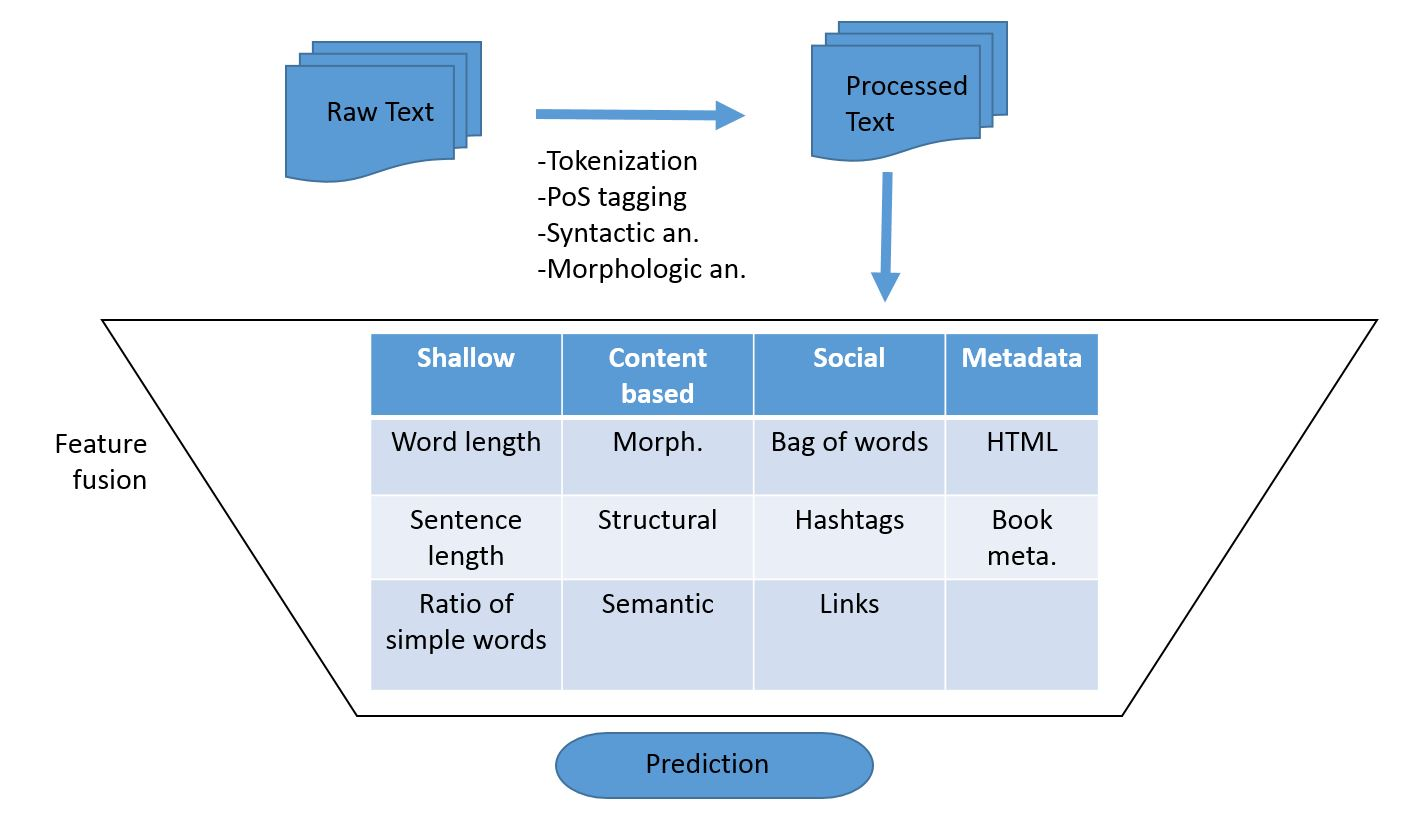
\includegraphics[width=\textwidth]{pipelineGraph}
\caption{MRAS}
\label{fig:pipeline}
\end{figure}

\subsection{Text processing}
%MRAS will used leveled corpora for learning from, i.e. a set documents that are labeled for its readability by experts. However, even if those documents are good to read by humans, they cannot be understood by machines, because they contain no structure. Therefore, the first step MRAS will always perform for a text is a processing step, where raw text is given structure and, therefore, value. This structure and information will later be used for extraction features that will help the system predict a readability score.\\
As the main focus of MRAS is to analyze text, we have identified different text processing methods and tools that will be used in its development. \textbf{Freeling NLP} \cite{padro12,padro10b} is a multilingual natural language processing (NLP) toolkit that supports 11 different languages. This tool solves common NLP tasks such as, tokenization, sentence detection, part of speech tagging or dependency parsing. \textbf{WordNet} is a lexical database that takes advantage of semantic relations between terms to build a graph that is very convenient for semantic analysis tasks. \textbf{Latent semantic analysis} is also a commonly used strategy  for semantic analysis, which takes advantage of concurrences among terms for determining similarities between them. All those tools, along with others that we will incorporate during the research process, will be used in the text processing step of MRAS.



%The tool that has been chosen for natural language processing is \textbf{Freeling NLP} \cite{padro12,padro10b}. Freeling is an open source Natural language processing library that supports 11 different languages. The tool solves common NLP tasks that will be used in the processing step, such as, tokenization, sentence detection, Part of speech tagging or dependency parsing. MRAS will also use other tools such as \textbf{WordNet} \cite{miller1995wordnet} or \textbf{Latent semantic analysis} \cite{landauer1998introduction} which will permit the analysis of the text in a semantic way. Each of this processes will be helpful for building certain features later.\\

%The \textbf{tokenization} is the base module for any NLP processing. Tokenization refers to taking a raw text and normalizing it into pieces that make text processing possible. This will also make possible, to implement tradition shallow features such as, Flesch–Kincaid \cite{flesch}. \\

%The \textbf{Part of speech} analysis determines the function each token has in the sentence. This, together with \textbf{dependency parsing} techniques, make possible the analysis of syntactic structures in the sentences.\\

%Other tools outside Freeling, such as \textbf{WordNet} or \textbf{Latent semantic analysis} techniques, will make possible to analyses texts at semantic level, for detecting structures that refer to concepts rather than to tokens themselves.\\



\subsection{Feature extraction}
Exploring features will be one of the main tasks of this thesis. MRAS should be able to extract a wide range of features that satisfy the needs of each language it will tackle. A general description of the categories of features that we expect to incorporate in MRAS is presented as follows:\\


\noindent
\textbf{Shallow features} \cite{flesch1948new,chall1995readability,albright1996readability} have historically shown to be of good use when predicting readability. Therefore, they will be incorporated into MRAS and used as a baseline for improvement. Sentence length, word length, or ratio of simple terms are examples of the features that will be included among this category.\\



\noindent
\textbf{Morphological features} capture how terms are formed from their root. Even if this  aspect is not relevant in some languages, such as English, it has been shown to be a strong predictor for readability scores in morphology rich languages such as Basque \cite{gonzalez2014simple}. Different morphological phenomena will be analyzed in order to create features in this category.\\

\noindent
\textbf{Structural features} are the ones that describe how a text is organized. They can both describe structure within the sentence (syntactical structure) or structure between sentences (pragmatical structure). Depth of the syntactic tree or ratios of different types of connectors between sentences are some examples of the features that are going to be explored under this category.\\

\noindent
\textbf{Semantic features} go beyond the tokens and structure of the text in order to analyse the concepts laying on it. %This permits to create an abstraction level that leave behind the dependence other features have respect to the text.
 Features such as concept density or concept follow-ability are some examples of the features that will be analyzed under this category.\\

\noindent
RA can be used in more than just plain text. Internet is evolving into a new social era and so are text resources. Increasingly more resources contain \textbf{social information}, such as hashtags, mentions, or links, a type of information that is usually ignored by readability formulas. We propose to investigate how the aforementioned information can be used for readability prediction.

\noindent
\textbf{Metadata} based features can be useful in environments where text access is limited (i.e. copyrighted material). An exploration of this type of features will also be done in order expand the types of texts MRAS can handle.



%named entities, childish not childish entities


%\subsection{Feature selection}

\subsection{Prediction}

Individually, each of the aforementioned features can only provide a rough estimate of the readability of a text. However, considering these features in-tandem can lead to a more accurate and robust readability assessment. Consequently, we will analyze different fusion strategies for MRAS, which will make possible to identify the most suitable strategies for readability prediction. The problem of assessing readability can be seen as a classification problem where a discrete categorical class needs to be predicted. Therefore, we would like to  explore different \textbf{classification} algorithms, such as bayesian networks \cite{nielsen2009bayesian} or support vector machines \cite{cortes1995support} for readability level prediction.  The RA task can also be seen as a \textbf{regression} problem, given that the class contains an inherent order on it. Therefore, we would also like to test different regression algorithms, including, but not limited to, linear regression \cite{neter1996applied} and logistic regression \cite{walker1967estimation}. Finally, we would also like to  explore a \textbf{hybrid} approach by using classification algorithms that take order in the class into account, such as the ordinal classification approach presented in \cite{frank2001simple}.





























\begin{comment}

The proposed method relies in two different areas of data science, Natural language processing and machine learning. Advantage of one or both areas is taken in each of the steps that conform the pipeline of the algorithm explained below.
\subsection{Pipeline description}
The pipeline of the algorithm if composed by the following steps: Texts processing, feature extraction, feature processing and prediction. A visual description of the general pipeline of the system can be seen on figure \ref{fig:pipeline}.  A more in-depth explanation of each step can be seen in the following sections.

\begin{figure}[ht]
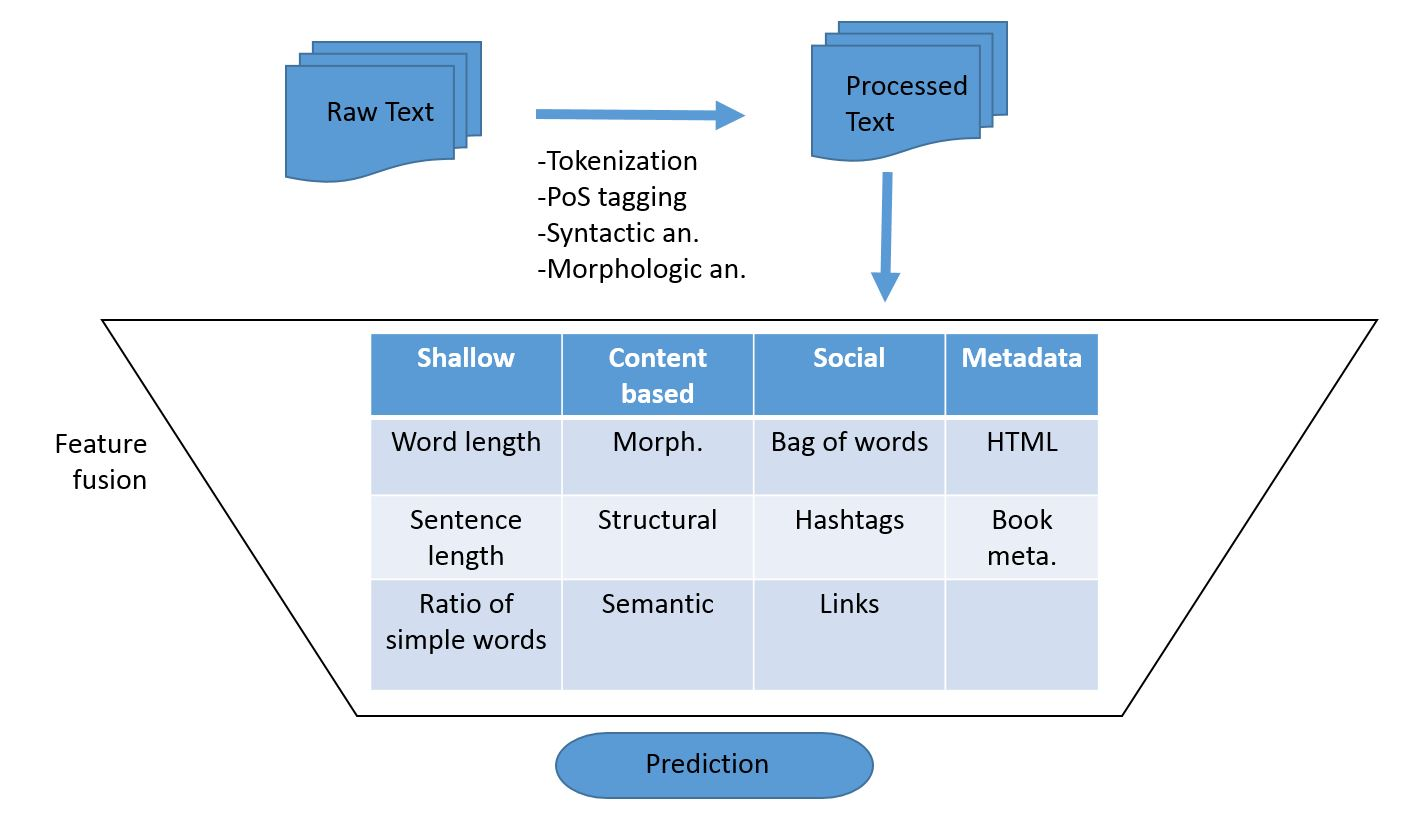
\includegraphics[width=0.2\textwidth]{pipelineGraph}
\caption{Description of MRAS}
\label{fig:pipeline}
\end{figure}

\subsection{Text processing}

The text processing step is the step where the raw text is given structure and, therefore, value. This structure and information will later be used for extraction features that will help the system predict a readability score.\\

The tool that has been chosen for natural language processing is Freeling NLP\cite{freelingNLP}. Freeling is an open source Natural language processing library that supports 11 different languages. The tool solves common NLP tasks, such as, Tokenization, sentence detection, Part of speech tagging or dependency parsing. Each of this processes will be helpful for building certain features later.\\

The \textbf{tokenization} is the base module for any NLP processing. Tokenization refers to taking a raw text and normalizing it into pieces that make text processing possible. This will also make possible, to implement tradition shallow features such as, Flesch–Kincaid \cite{flesch}. \\

The \textbf{Part of speech} analysis determines the function each token has in the sentence. This, together with \textbf{dependency parsing} techniques, make possible the analysis of syntactic structures in the sentences.\\

Other tools outside Freeling, such as \textbf{WordNet} or \textbf{Latent semantic analysis} techniques, will make possible to analyses texts at semantic level, for detecting structures that refer to concepts rather than to tokens themselves.\\


\subsection{Feature extraction}




This section describes the features proposed for the system. These features range from the most simple and commonly used ones such as the shallow features, to a more complex set of features such as the ones base on semantics.

\subsubsection*{Shallow features}
\subsubsection*{Part of Speech tags}

\subsubsection*{N-grams}

...

Description of all the features used. Why should this feature be valuable, give hypotheses and intuition behind the use of each feature. Give examples when needed.

\subsection{Feature processing and selection}
Describe algorithms used for feature processing and selection, why should they help get better results?

\subsection{Learning and prediction}
Describe algorithms for learning and prediction. Pros an cons of each algorithm, why should this algorithm adapt better to our problem?
\end{comment}







\section{Evaluation}

Even if MRAS is designed to be language independent, for practical purposes the evaluation will only be conducted in three languages that we think can faithfully represent the diversity of existing languages. For this purpose, we have chosen a germanic, a romance, and a pre-indioeuropean language, i.e. English, Spanish, and Basque respectively.


\subsection{Datasets}
The ideal dataset for developing MRAS would be a multilingual leveled dataset that would contain the exact same documents written in different languages, as well as human judgments, in terms of readability scores for each document. However, to the best of our knowledge, such a dataset does not currently exist. Consequently, we have identified various sets of leveled documents for each individual language that can suit MRAS' needs and can be used for evaluation purposes. Details on the datasets considered for evaluation purposes can be seen in Table \ref{table:datastetTable}.




% Please add the following required packages to your document preamble:
% \usepackage{multirow}
% \usepackage{graphicx}
\begin{table}[h]
\centering
\resizebox{\textwidth}{!}{%
\begin{tabular}{l|l|l|}
\cline{2-3}
                                                        & \textbf{Dataset}   & \textbf{Description}                                         \\ \hline
\multicolumn{1}{|l|}{\multirow{4}{*}{\textbf{English}}} & Lexile \cite{datasetEuOther1}            & Contains book titles associated with its readability level   \\ \cline{2-3} 
\multicolumn{1}{|c|}{}                                  & Stantarized tests \cite{datasetEnExams1,datasetEnExams2} & Tests for English level, they contain various texts per test \\ \cline{2-3} 
\multicolumn{1}{|c|}{}                                  & Other \cite{datasetEnOther1,datasetEnOther2,datasetEnOther3}             & News for kids, exercises for learning English                \\ \hline




\multicolumn{1}{|l|}{\multirow{2}{*}{\textbf{Spanish}}} & Lexile  \cite{datasetEuOther1}           & Contains book titles associated with its readability level   \\ \cline{2-3} 
\multicolumn{1}{|l|}{}                                  & Learning resources \cite{datasetEsOther1,datasetEsOther2,datasetEsOther3} & Various exercises for learning Spanish                       \\ \hline


\multicolumn{1}{|l|}{\textbf{Basque}}                   & Learning resources \cite{datasetEuOther1} & Various exercises for learning Basque                        \\ \hline
\multicolumn{1}{|l|}{\textbf{Multilingual}}                   & Parallel corpus \cite{datasetParallel1}  & Contains same texts translated into Spanish                        \\
\multicolumn{1}{|l|}{}                   &   &  and English \\
 \hline
\end{tabular}%
}
\caption{Data resources identified for MRAS development and validation}
\label{table:datastetTable}
\end{table}


\begin{comment}
\subsubsection{English}
\begin{itemize}
\item \textbf{Lexile} is an online resource containing titles of books with a readability score assigned. Even if the whole content of books is not available, snippets of text can be obtained from different online resources that will be explored.
\item \textbf{Standarized English tests} institutions, such as Cambridge or the British council, make sample test contents publicly available for students to test themselves. A significant dataset can be created using the texts contained in them.
\item \textbf{Other online resources}  that can be used for MRAS development have been identified. Those resources vary from other online available children books\footnote{https://www.readinga-z.com/books/leveled-books/} to leveled news and articles\footnote{http://www.breakingnewsenglish.com/news-for-kids.html}\footnote{http://www.newsinlevels.com/} for children.
\end{itemize}
\subsubsection{Spanish}
\begin{itemize}
\item \textbf{Lexile}: Same as for English an smaller version of Lexile database is available for Spanish too.
\item \textbf{Various learning materials} \footnote{http://cvc.cervantes.es/aula/lecturas/} \footnote{http://aprenderespanol.org/lecturas/lecturas-ejercicios.html} \footnote{http://www-k6.thinkcentral.com/content/hsp/reading/Senderos/na/common/
online\_senderos\_libros\_graduables\_para\_lectores/senderos\_SE/launch.html} have also been identified that could be used as part of the dataset. Those resources mostly contain reading materials that are aimed at learning Spanish.
\end{itemize}
\subsubsection{Basque}

\begin{itemize}
\item \textbf{Ikasbil} is an online resource for learning Basque that contains different media contents, such as articles, videos, or audio contents. Every content is leveled given its complexity.
\end{itemize}

\subsubsection{Multilingual}
\begin{itemize}
\item A \textbf{parallel corpus} \footnote{http://albalearning.com/audiolibros/textosparalelos.html} for Spanish and English have also been identified, that contain exact same documents translated into the two languages.
\end{itemize}

\end{comment}


\subsection{Metrics}
The performance of MRAS will be evaluated by means of (1) common classification evaluation methods, such as absolute error \cite{croft2010search}, (2) regression evaluation methods such as MSE (Mean Square Error) \cite{croft2010search} and (3) methods common in the readability assessment domain, such as adjacent accuracy \cite{franccois2012ai}. 

\subsection{Overall Assessment}
The study and performance analysis of this thesis will aim at answering the following questions:
\begin{itemize}

\item Which learning model performs better for MRAS? Which feature subset?
\item Which features add more value in terms of predicting readability? Do they add same value for each language?
\item How does MRAS perform compared to baseline shallow feature based formulas? and compared to state of the art systems?
\item Would MRAS give the same prediction for a text that is translated manually into another language? and for a text that is automatically translated?
\item How efficiently can MRAS predict the readability levels of written text in a language for which it has not been trained? If we train MRAS for two languages can we use it to predict the readability of a text in a third one?
\item If we have a really small dataset for one language, would adding more data from another language improve the prediction results of the first one?

\end{itemize}


%\begin{itemize}

%\item Which features add the most value? Correlation, information gain etc.

%\item Do features correlate similarly with the readability score for each language?

%\item Feature preprocessing, does it help?
%	\begin{itemize}
%	\item Discretization
%	\item Feature subset selection techniques
%	\end{itemize}
	
%\item Comparison of learning models, which learning model fits best the problem?
%	\begin{itemize}
%	\item KNN
%	\item Bayesian models
%	\item SVM
%	\item Neural network
%	\item Regression (Adding a sense of order in class values)
%	\item Ordinal classification (Adding a \textbf{stronger} sense of order in class values)
%	\end{itemize}

%\item \textbf{Comparison} of the system vs \textbf{baselines} such as fleish for each language individually.

%\item Comparison \textbf{vs state of the art} systems for each language.

%\item Multi vs monolingual
%\item If we take a bilingual corpus, does the system predict same values? And if we take a text and translate it to another language? Does the readability values maintain using an automatic translator?
%\item Can we predict the readability of a language, even if the model is not trained for that especific language? Can we predict basque readability even only training for english and spanish? could we predict italian or catalonian if we train our system in spanish?(hypothetically easier, because they contain similar roots)
%\end{itemize}


\section{Proposed schedule}
For conducting the research proposed in this manuscript in a timely manner, we define the milestones shown in Table \ref{table:schedule}.

% Please add the following required packages to your document preamble:
% \usepackage{graphicx}
\begin{table}[h!]
\centering
%\resizebox{\textwidth}{!}{%
\begin{tabular}{|c|l|}
\hline
\textbf{Date} & \textbf{Milestone}                                  \\ \hline
April 2016    & Gather existing datasets for design and development \\ \hline
May 2016    & Feature Exploration                                 \\ \hline
%April 2016    & Feature Exploration: Content based features         \\ \hline
%April 2016    & Feature Exploration: Social features                \\ \hline
June 2016    & Feature fusion                                      \\ \hline
July 2016    & Experiments                                         \\ \hline
July 2016    & Thesis draft                                        \\ \hline
August 2016    & Defense                                             \\ \hline
\end{tabular}%
%}
\caption{Proposed schedule}
\label{table:schedule}
\end{table}

\newpage

\bibliography{bibliography}{}
\bibliographystyle{abbrv}

\includepdf[pages={4}]{proposalForm.pdf}

\end{document}